\documentclass[a4paper, 12pt]{ctexart}

%================= 宏包引入 =================%
\usepackage{geometry} % 页面边距设置
\geometry{left=2.5cm, right=2.5cm, top=2.5cm, bottom=2.5cm}
\usepackage{amsmath, amssymb, amsfonts} % 数学公式与符号
\usepackage{graphicx} % 插入图片
\usepackage{float} % 浮动体控制 (如 H 参数)
\usepackage{caption} % 图表标题设置
\usepackage{subcaption} % 子图设置
\usepackage{booktabs} % 三线表
\usepackage{listings} % 代码高亮
\usepackage{xcolor} % 颜色支持
\usepackage{hyperref} % 超链接支持

%================= 样式与代码高亮设置 =================%
\hypersetup{
    colorlinks=true,
    linkcolor=black,
    filecolor=blue,      
    urlcolor=blue,
    citecolor=black,
}

% 定义 MATLAB 代码颜色
\definecolor{mygreen}{RGB}{28,172,0}
\definecolor{mylilas}{RGB}{170,55,241}
\definecolor{backcolour}{rgb}{0.96,0.96,0.94}

\lstset{
    language=Matlab,
    backgroundcolor=\color{backcolour},
    basicstyle=\ttfamily\small,
    breaklines=true,
    keywordstyle=\color{blue}\bfseries,
    stringstyle=\color{mylilas},
    commentstyle=\color{mygreen},
    showstringspaces=false,
    numbers=left,
    numberstyle=\tiny\color{gray},
    stepnumber=1,
    frame=single,
    rulecolor=\color{black!30},
    tabsize=4,
    % 中文注释支持
    extendedchars=false
}

% 图表标题格式
\captionsetup{font=small, labelfont=bf}

%================= 首页与标题信息 =================%
\title{\vspace{2cm}\textbf{\Huge 倒立摆系统状态观测器设计实验报告}}
\author{\Large 实验人员：PB23051023 杜晓阳， PB23061299 周奕衡}
\date{\large 实验日期：2025年04月24日}

\begin{document}

\maketitle
\thispagestyle{empty} % 首页不显示页码

\newpage
\setcounter{page}{1}

%================= 正文部分 =================%
\section{实验目的}
本实验旨在针对直线一级倒立摆系统，在系统状态变量不完全可测的实际条件下，设计状态观测器以实现对全系统状态的估计。具体目标包括：
\begin{enumerate}
    \item 掌握基于极点配置法的全维状态观测器设计方法。
    \item 了解并初步探索卡尔曼观测器（滤波器）在噪声环境下的应用。
    \item 通过仿真与理论分析，比较两种状态估计方法的特性，验证观测器对于实现基于状态反馈控制的重要性。
\end{enumerate}

\section{实验原理}
当采用状态反馈控制律 $u = -Kx$ 时，需要获取全部状态变量 $x$。在实际倒立摆系统中，小车速度 $\dot{x}$ 杆角速度 $\dot{\phi}$ 通常难以直接精确测量。状态观测器通过利用可直接测量的输出量（如小车位移 $x$ 和摆杆角度 $\phi$）及已知的系统模型，在线估计出全部状态。

\subsection{全维状态观测器原理}
对于线性系统：
\begin{equation}
    \dot{x} = Ax + Bu, \quad y = Cx
\end{equation}
其全维状态观测器的动态方程为：
\begin{equation}
    \dot{\hat{x}} = A\hat{x} + Bu + H(y - C\hat{x}) = (A-HC)\hat{x} + Bu + Hy
\end{equation}
其中，$\hat{x}$ 为状态估计值，$H$ 为观测器增益矩阵。估计误差 $e = x - \hat{x}$ 的动态方程为 $\dot{e} = (A-HC)e$。若系统 $(A, C)$ 可观测，则可通过设计 $H$ 任意配置 $(A-HC)$ 的特征值（即观测器极点），使估计误差以指数速率收敛至零。为保证估计快速跟踪真实状态，观测器极点通常被配置在状态反馈闭环极点的左侧（实部更负）。

\subsection{卡尔曼观测器原理简述}
卡尔曼滤波器是一种最优状态估计器，适用于系统存在过程噪声和测量噪声的场合。其核心思想是通过预测和更新两个步骤，最小化状态估计的均方误差。对于离散化后的系统模型：
\begin{equation}
\begin{aligned}
    x_{k} &= F x_{k-1} + G u_{k-1} + w_{k-1} \\
    y_k &= C x_k + v_k
\end{aligned}
\end{equation}
其中 $w$ 和 $v$ 分别为均值为零、协方差矩阵为 $Q$ 和 $R$ 的过程噪声和测量噪声。卡尔曼滤波器通过递归算法，提供系统状态在统计意义下的最优估计 $\hat{x}_k$。在噪声环境下，其性能通常优于标准的确定性观测器。

\begin{figure}[H]
    \centering
    % 注意：此处将路径替换为了文件名，请确保图片在同级目录下
    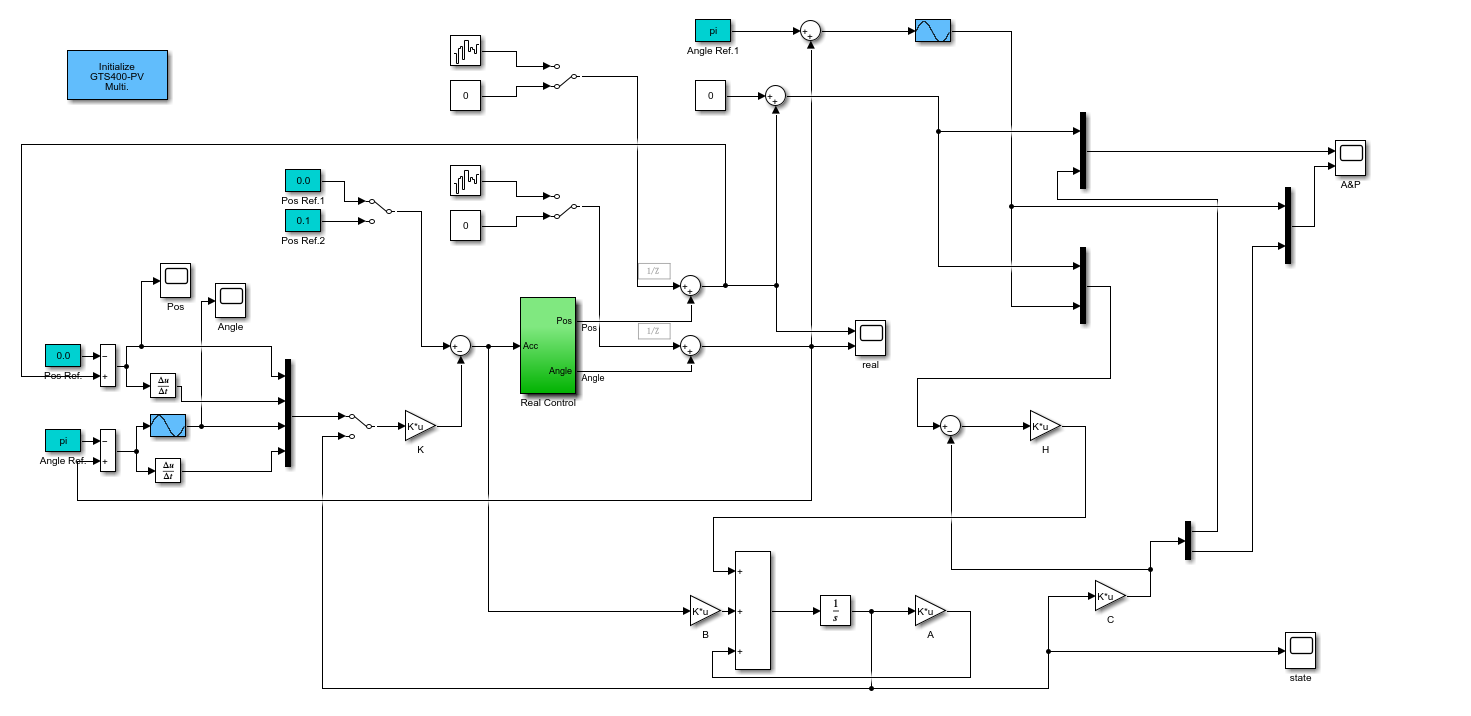
\includegraphics[width=0.85\textwidth]{system.png}
    \caption{MATLAB实际控制程序图}
\end{figure}

\section{实验内容与步骤}

\subsection{系统建模}
直线一级倒立摆系统的线性化状态空间模型如下：
\begin{equation}
\begin{aligned}
    A &= \begin{bmatrix}
    0 & 1 & 0 & 0 \\
    0 & 0 & 0 & 0 \\
    0 & 0 & 0 & 1 \\
    0 & 0 & 29.4 & 0
    \end{bmatrix}, \quad
    B = \begin{bmatrix}
    0 \\ 1 \\ 0 \\ 3
    \end{bmatrix} \\[8pt]
    C &= \begin{bmatrix}
    1 & 0 & 0 & 0 \\
    0 & 0 & 1 & 0
    \end{bmatrix}, \quad
    D = \begin{bmatrix}
    0 \\ 0
    \end{bmatrix}
\end{aligned}
\end{equation}
状态变量为 $x = [x, \dot{x}, \phi, \dot{\phi}]^T$，输出变量为 $y = [x, \phi]^T$。

\subsection{状态反馈控制器设计}
首先，为闭环系统配置期望极点，设计状态反馈矩阵 $K$。根据文档，选取的闭环极点为：
\begin{equation}
    \mu_1 = -3, \quad \mu_2 = -4, \quad \mu_3 = -4+5i, \quad \mu_4 = -4-5i
\end{equation}
对应的期望特征方程为：
\begin{equation}
    s^4 + 15s^3 + 109s^2 + 383s + 492 = 0
\end{equation}
利用极点配置方法，计算得到状态反馈增益矩阵为：
\begin{equation}
    K = \begin{bmatrix} -13.8776 & -12.1769 & 53.0925 & 9.7256 \end{bmatrix}
\end{equation}

\subsection{确定性状态观测器设计}
根据分离原理，独立设计状态观测器。为使观测器动态快于闭环系统，将观测器极点配置在：
\begin{equation}
    \lambda_1 = -6, \quad \lambda_2 = -8, \quad \lambda_3 = -8+5i, \quad \lambda_4 = -8-5i
\end{equation}
通过极点配置（例如使用 \texttt{place} 或 \texttt{acker} 函数），求解得到观测器增益矩阵 $H$ 为：
\begin{equation}
    H = \begin{bmatrix}
    18.0628 & -3.7080 \\
    81.3742 & -29.2187 \\
    1.8746 & 15.9372 \\
    9.7227 & 90.2045
    \end{bmatrix}
\end{equation}

\subsection{卡尔曼观测器设计}
文档中指出，卡尔曼观测器的设计基于前述相同的系统模型 $(A, B, C, D)$。关键步骤包括：
\begin{enumerate}
    \item \textbf{系统离散化}：将连续系统模型转换为离散时间模型，得到状态转移矩阵 $F$ 和输入矩阵 $G$。
    \item \textbf{噪声建模}：设定或辨识过程噪声协方差矩阵 $Q$ 和测量噪声协方差矩阵 $R$。
    \item \textbf{算法实现}：实现卡尔曼滤波的预测与更新递归迭代算法。在仿真中，此部分被封装成模块。
\end{enumerate}

\subsection{仿真实验}
搭建包含被控对象、状态反馈控制器和两种观测器的综合仿真模型（结构可参考文档中提到的“matlab框架结构”）。进行以下对比实验：
\begin{enumerate}
    \item \textbf{无噪声环境下状态观测器性能验证}：测试所设计的确定性观测器的状态跟踪效果。
    \item \textbf{噪声环境下两种观测器性能对比}：在系统输出端添加噪声，比较确定性观测器与卡尔曼观测器的状态估计精度及闭环系统的控制性能。
\end{enumerate}

\section{实验结果与分析}

\subsection{确定性状态观测器性能（无噪声）}
在无噪声的理想情况下，设计的观测器能够快速、准确地估计出系统的全部状态（包括不可直接测量的 $\dot{x}$ 和 $\dot{\phi}$）。基于观测状态的反馈控制能使倒立摆系统稳定，验证了极点配置法设计观测器的有效性。


\begin{figure}[H]
    \centering
    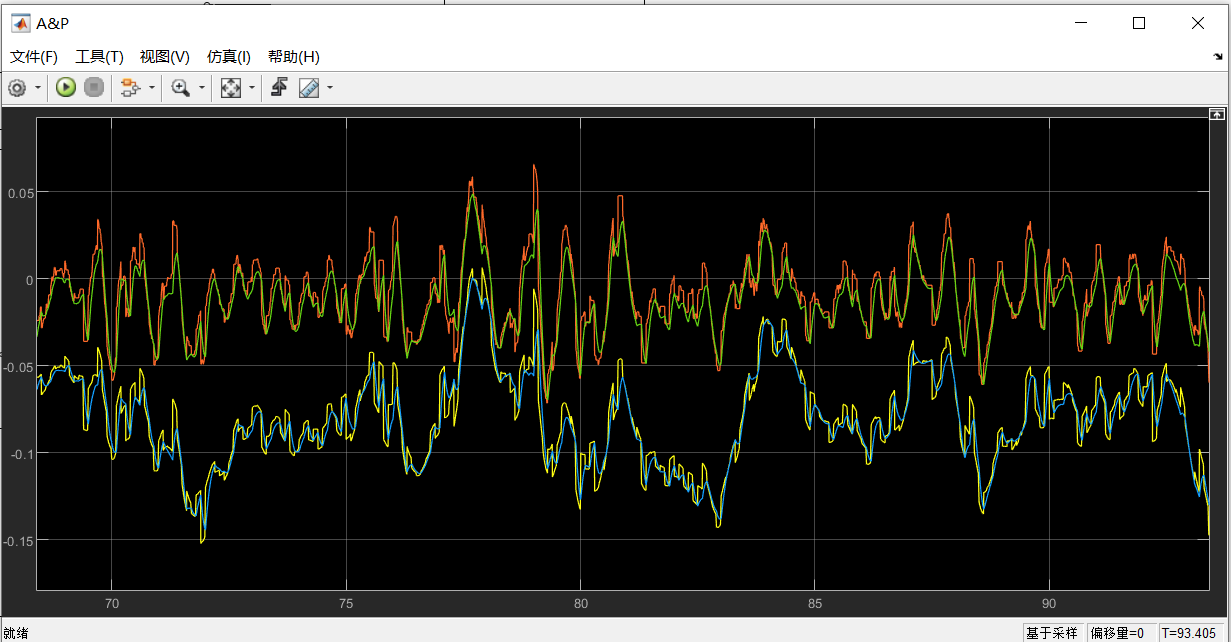
\includegraphics[width=0.85\textwidth]{real&obs.png}
    \caption{实际效果图}
\end{figure}

\begin{figure}[H]
    \centering
    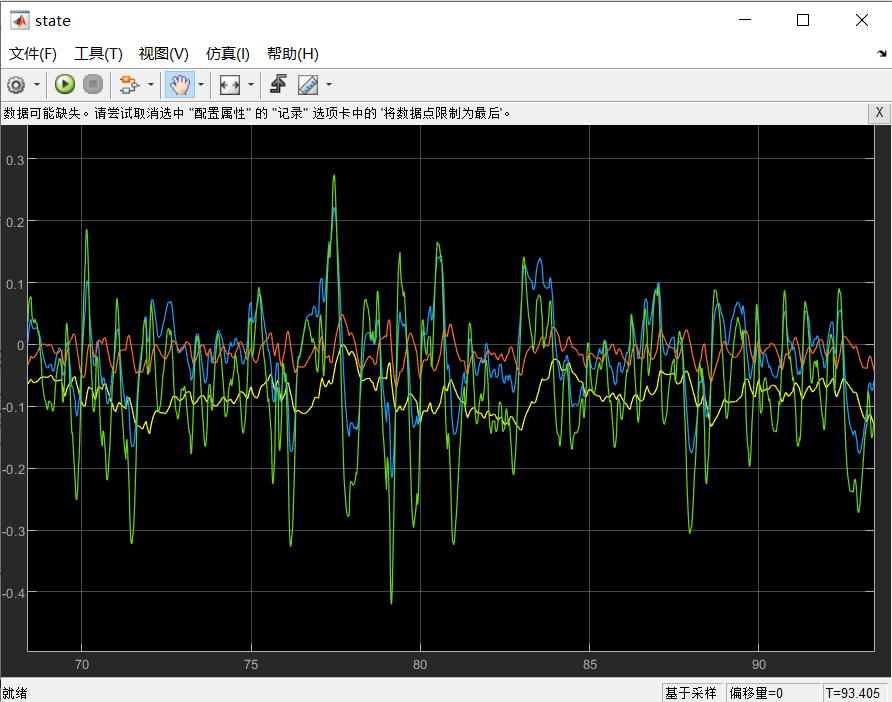
\includegraphics[width=0.85\textwidth]{obs.png}
    \caption{选取的四种状态变量的实时控制情况}
\end{figure}

\begin{figure}[H]
    \centering
    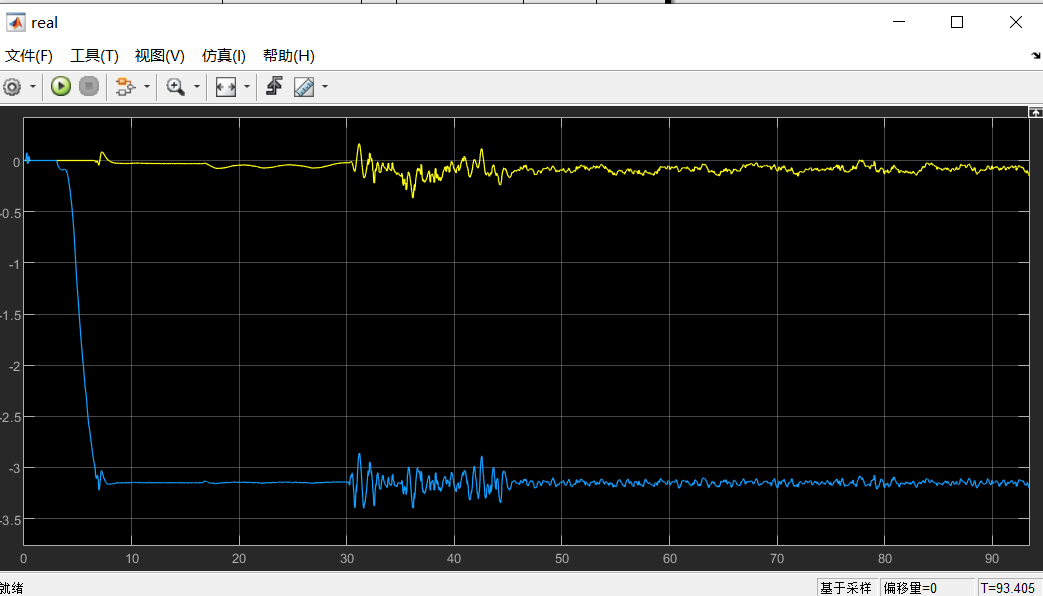
\includegraphics[width=0.85\textwidth]{real.png}
    \caption{反映角度与位移的变化情况，其中中间时刻加入扰动}
\end{figure}
\subsection{卡尔曼观测器性能}
展示了卡尔曼观测器的仿真结果和实际控制效果。
\begin{enumerate}
	\item \textbf{仿真结果}：在存在噪声的仿真环境中，卡尔曼观测器能够有效地滤除噪声，提供平滑、准确的状态估计，从而使闭环系统保持良好的稳定性能。
	\item \textbf{实际控制效果}：结论指出，“卡尔曼在有噪声的情况下依旧展现出了很好的控制效果”。这表明将卡尔曼滤波器应用于倒立摆状态估计，能显著提升系统在真实噪声环境下的鲁棒性和控制品质。
\end{enumerate}

\subsection{两种观测器的简要对比分析}
\begin{itemize}
    \item \textbf{确定性观测器}：设计简单，概念直观，通过配置极点可直接决定状态估计的收敛速度。但在系统存在显著噪声时，其估计效果会下降，因为它没有内嵌的噪声统计模型和最优滤波机制。
    \item \textbf{卡尔曼观测器}：作为一种最优估计算法，它显式地考虑了过程噪声和测量噪声，通过最小化估计误差的协方差来提供最优估计。因此在噪声环境下，其估计精度和鲁棒性通常优于确定性观测器，但需要已知或能较准确设定噪声的统计特性（$Q$ 和 $R$ 矩阵）。
\end{itemize}

\section{实验总结与思考}
\begin{enumerate}
    \item \textbf{实验成果}：本次实验成功地为倒立摆系统设计了基于极点配置的确定性状态观测器和卡尔曼观测器。仿真结果表明，两者均能实现系统状态的重构，从而使基于全状态反馈的控制策略得以实施。
    \item \textbf{核心认识}：观测器是现代控制理论连接理想设计与工程实践的关键桥梁。它解决了状态不完全可测的难题，使得最优控制（如LQR）、鲁棒控制等基于状态反馈的高级算法得以在实际系统中应用。
    \item \textbf{性能差异}：在无噪声或噪声很小的理想环境下，合理配置极点的确定性观测器已能满足需求。然而，在存在显著噪声的实际系统中，卡尔曼滤波器因其最优滤波特性，能提供更优的状态估计，从而带来更好的整体控制性能。这解释了在高端或复杂控制系统中卡尔曼滤波器及其变种被广泛使用的原因。
    \item \textbf{实验扩展}：本次实验主要完成了观测器的设计与初步验证。未来可进一步深入分析不同极点配置对观测器动态性能及鲁棒性的影响，以及研究在 $Q$、$R$ 矩阵不准确时卡尔曼滤波器的性能变化，或尝试更先进的非线性观测器与滤波器设计。
\end{enumerate}

\vspace{1em}
\noindent\textbf{思考题：在添加噪声和不添加噪声的情况下，对比分析有无观测器时的控制效果；}

\noindent 其核心结论可概括为：观测器的作用随噪声环境变化而不同。在无噪声的理想情况下，观测器的主要价值在于解决状态不可直接测量的问题，使基于状态反馈的先进控制方法得以实现，其控制效果接近状态完全可测的理想情况。然而，在实际存在测量噪声的情况下，观测器的作用至关重要且发生质变：若无观测器，含噪声的测量信号会直接干扰控制器，导致控制指令抖动、性能恶化甚至失稳；而引入设计良好的观测器（如卡尔曼滤波器）后，它不仅能重构不可测状态，更关键的是能依据系统模型对测量噪声进行最优滤波，为控制器提供相对“干净”的状态估计，从而显著提升系统在噪声环境下的控制精度、稳定性和整体鲁棒性。因此，观测器是从理论设计走向工程应用的关键，尤其在存在噪声的实际系统中不可或缺。

\newpage
\section*{附录：代码与运行结果}

\subsection*{MATLAB 代码}
\begin{lstlisting}
clear; clc;

%% 系统参数定义
A = [0  1   0    0;
     0  0   0    0;
     0  0   0    1;
     0  0  29.4  0]; 

B = [0; 1; 0; 3];

C = [1 0 0 0;   % 小车位置
     0 0 1 0];  % 摆杆角度

desired_poles=[-3,-4,-5+3i,-5-3i];

syms s k1 k2 k3 k4 real
K=[k1,k2,k3,k4];
Ac=A-B*K;

f = det(s*eye(4)-Ac);
coeff_cl=coeffs(f,s,'All');

coeff_des=poly(desired_poles);
eqns = coeff_cl(2:end) == coeff_des(2:end);

sol= solve(eqns,K);
K_num= double([sol.k1,sol.k2,sol.k3,sol.k4]);

fprintf('待定法K=[%.4f,%.4f,%.4f,%.4f]\n',K_num);

closed_poles = eig(A -B*K_num);
disp(closed_poles); 

%% 观测器设计
desired_poles_obs=[-6,-8,-10+3i,-10-3i];
H=place(A',C',desired_poles_obs)';

fprintf('H=\n');
disp(H);
\end{lstlisting}

\subsection*{运行结果}
\begin{lstlisting}[language={}, frame=none, backgroundcolor=\color{white}]
待定法K=[-13.8776,-12.1769,53.0925,9.7256]

  -5.0000 + 3.0000i
  -5.0000 - 3.0000i
  -4.0000 + 0.0000i
  -3.0000 + 0.0000i

H=
   18.0628   -3.7080
   81.3742  -29.2187
    1.8746   15.9372
    9.7227   90.2045
\end{lstlisting}

\end{document}